\section{ЗАДАНИЕ}

\begin{enumerate}
    \item Максимум из двух чисел
        \begin{enumerate}
            \item без использования отсечения,
            \item с использованием отсечения;
        \end{enumerate}
    \item Максимум из трех чисел
        \begin{enumerate}
            \item без использования отсечения,
            \item с использованием отсечения
        \end{enumerate}
\end{enumerate}


\begin{lstlisting}[caption=Максимум 2 чисел]
predicates
	maxWithCut(integer, integer, integer).
	maxWoutCut(integer, integer, integer).

clauses
	% Max of two numbers with using cut
	maxWithCut(A, B, Max) :- A > B, Max = A, !.
	maxWithCut(_, B, Max) :- Max = B.

	% Max of two numbers without using cut
	maxWoutCut(A, B, Max) :- A > B, Max = A.
	maxWoutCut(A, B, Max) :- A <= B, Max = B.

goal
	write("maxWithCut of (3, 2):\t"),
	maxWithCut(3, 2, Max);

	write("maxWithCut of (1, 2):\t"),
	maxWithCut(1, 2, Max);
	
	write("maxWithCut of (1, 1):\t"),
	maxWithCut(1, 1, Max);

	write("maxWoutCut of (3, 2):\t"),
	maxWoutCut(3, 2, Max);

	write("maxWoutCut of (1, 2):\t"),
	maxWoutCut(1, 2, Max);

	write("maxWoutCut of (1, 1):\t"),
	maxWoutCut(1, 1, Max).
\end{lstlisting}

\begin{lstlisting}[caption=Максимум 3 чисел]
predicates
	maxWithCut(integer, integer, integer, integer).
	maxWoutCut(integer, integer, integer, integer).

clauses
	% Max of three numbers with using cut
	maxWithCut(A, B, C, Max) :- A > B, A > C, Max = A, !.
	maxWithCut(_, B, C, Max) :- B > C, Max = B, !.
	maxWithCut(_, _, C, Max) :- Max = C.

	% Max of three numbers without using cut
	maxWoutCut(A, B, C, Max) :- A >= B, A >= C, Max = A.
	maxWoutCut(A, B, C, Max) :- B > A, B >= C, Max = B.
	maxWoutCut(A, B, C, Max) :- C > A, C > B, Max = C.

goal
	write("maxWithCut of (1, 2, 3):\t"),
	maxWithCut(1, 2, 3, Max);
	write("maxWithCut of (3, 2, 1):\t"),
	maxWithCut(3, 2, 1, Max);
	write("maxWithCut of (4, 2, 4):\t"),
	maxWithCut(4, 2, 4, Max);
	write("maxWithCut of (1, 5, 3):\t"),
	maxWithCut(1, 5, 3, Max);
	
	write("maxWoutCut of (1, 2, 3):\t"),
	maxWoutCut(1, 2, 3, Max);
	write("maxWoutCut of (3, 2, 1):\t"),
	maxWoutCut(3, 2, 1, Max);
	write("maxWoutCut of (4, 2, 4):\t"),
	maxWoutCut(4, 2, 4, Max);
	write("maxWoutCut of (1, 5, 3):\t"),
	maxWoutCut(1, 5, 3, Max).
\end{lstlisting}

\section{РЕЗУЛЬТАТЫ РАБОТЫ}

\begin{figure}[H]
    \centering
    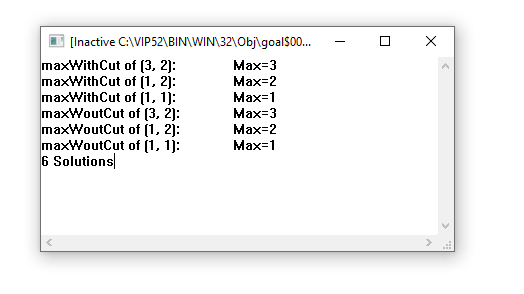
\includegraphics[scale=0.8]{img/max2.png}
    \caption{Максимум 2 чисел}
\end{figure}

\begin{figure}[H]
    \centering
    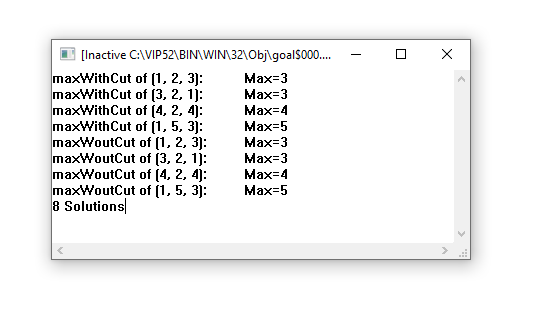
\includegraphics[scale=0.8]{img/max3.png}
    \caption{Максимум 3 чисел}
\end{figure}
